\documentclass[a4paper,10pt]{article}
\usepackage{longtable}
\usepackage[utf8]{inputenc}
\usepackage{url}
\usepackage{hyperref}
\usepackage{listings}
\usepackage{color}
\usepackage{verbatim}
\definecolor{grey}{rgb}{0.9,0.9,0.9}
\usepackage{float}
\usepackage{graphicx}
\usepackage{fancyhdr}
\pagestyle{fancy} % voir si laisse ce style ou pas ?
%\usepackage[top=2.5cm,bottom=2.5cm,right=2.5cm,left=2.5cm]{geometry}
\usepackage[right=4cm,left=4cm]{geometry}
\lstset{
language=C++,
basicstyle=\footnotesize\fontfamily{pcr},
backgroundcolor=\color{grey},
numbers=left,
numberstyle=\tiny,
numbersep=5pt,
showstringspaces=false,
tabsize=2,
breaklines=true
}
%\usepackage{titlesec}
%\titleformat{\section}[frame]{\normalfont\Huge\bfseries}{\thesection}{0.5em}{}
%\titleformat{\subsection}[block]{\normalfont\LARGE\bfseries}{\thesubsection}{1em}{}
%\titleformat{\subsubsection}[block]{\normalfont\large\bfseries}{\thesubsubsection}{1em}{}


% Title Page
\title{INFO-F403 Introduction to Language Theory and Compilation}
\author{Chapeaux Thomas\\Dagnely Pierre}

\begin{document}
\maketitle

Le but du projet était de construire un compilateur d'une version simplifiée de Perl en ASM/ARM devant tourner dans une architecture Android.\\

La première partie de ce rapport se concentrera sur l'analyse du language, c'est-à-dire la définition des tokens et de la grammaire LL(1) correspondante, ainsi que la table d'action et les contraintes que nous avons imposé lors de la transformation en LL(1).\\

Ensuite, nous décrirons notre parser qui transforme un fichier .perl en un AST.\\

Finalement, nous expliquerons la génération du code ASM/ARM.

\pagebreak
%%%%%%%%%%%%%%%%%%%%%%%%%%%%%%%%%%%%%%%%%%%%%%%%%%%%%%%%%%%%%%%%%%%%%%%%%%%%%%%%%%%%%%%%%%%%%%%%%%%%%%%%%%%%%%%%%%%%%%%%%%%%%%%%%%%%%%%%%
%%
%%
%%	Quenstion 1 : Lexèmes
%%
%%
%%%%%%%%%%%%%%%%%%%%%%%%%%%%%%%%%%%%%%%%%%%%%%%%%%%%%%%%%%%%%%%%%%%%%%%%%%%%%%%%%%%%%%%%%%%%%%%%%%%%%%%%%%%%%%%%%%%%%%%%%%%%%%%%%%%%%%%%%%

\section{Language}
\subsection{Lexèmes}

Définition des tokens~\\

\begin{tabular}{cc}

\begin{tabular}{|c|l|}
\hline
Lexical units  		& regular expressions \\ \hline
INT					& ([0-9])* \\ \hline
FLOAT				& ([0-9])*.DOT.([0-9])* \\ \hline
BOOL				& (0+1+true+false+'') \\ \hline
STRING				& '.([A-Za-z]+[0-9])*.'  \\ \hline
FAC					& ! \\ \hline
MUL					& * \\ \hline
DIV					& / \\ \hline
MINUS				& - \\ \hline
ADD					& + \\ \hline
LT					& $<$ \\ \hline
GT					& $>$ \\ \hline
LE					& $<=$ \\ \hline
GE					& $>=$ \\ \hline
EQUIV				& == \\ \hline
DIF					& != \\ \hline
AND					& \&\& \\ \hline
OR					& $||$ \\ \hline
NOT					& not \\ \hline
LT-S				& lt \\ \hline
GT-S				& gt \\ \hline
LE-S				& le \\ \hline
GE-S				& ge \\ \hline
EQ-S				& eq \\ \hline 
NE-S				& ne \\ \hline
\end{tabular}

&

\begin{tabular}{|c|l|}
\hline
Lexical units  		& regular expressions \\ \hline
EQUAL				& = \\ \hline
DOT					& . \\ \hline
SEMICOLON			& ; \\ \hline
COMA				& , \\ \hline
OPEN-PAR			& ( \\ \hline
CLOSE-PAR			& ) \\ \hline
OPEN-BRAC			& \{ \\ \hline
CLOSE-BRAC			& \} \\ \hline
OPEN-COND			& IF \\ \hline
CLOSE-COND 			& ELSE \\ \hline
ADD-COND			& ELSIF \\ \hline
NEG-COND			& UNLESS \\ \hline
RET					& return \\ \hline
FUNCT-DEF			& SUB \\ \hline
ID					& STRING \\ \hline 
FUNCT-NAME			& \&.STRING \\ \hline
PERL-DEF			& defined  \\ \hline
PERL-INT			& int  \\ \hline
PERL-LENG			& length  \\ \hline
PERL-SCAL			& scalar  \\ \hline
PERL-SUBS			& substr  \\ \hline
PERL-PRIN			& print\\ \hline
COMM				& \#.STRING \\ \hline
VARIABLE			& \$.STRING \\ \hline


\end{tabular}
\end{tabular}
~\\

Remarques :
\begin{itemize}
\item Le lexème COMA peut définir l'opérateur virgule ou juste une virgule entre deux paramètres. Le lexème est le même mais le parser l'interpretera différemment.\\
\item Les lexèmes de type COMM (commentaire) sont supprimés avant de faire l'analyse lexicale
\end{itemize}


\pagebreak
%%%%%%%%%%%%%%%%%%%%%%%%%%%%%%%%%%%%%%%%%%%%%%%%%%%%%%%%%%%%%%%%%%%%%%%%%%%%%%%%%%%%%%%%%%%%%%%%%%%%%%%%%%%%%%%%%%%%%%%%%%%%%%%%%%%%%%%%%
%%
%%
%%	Quenstion 2 : Automates
%%
%%
%%%%%%%%%%%%%%%%%%%%%%%%%%%%%%%%%%%%%%%%%%%%%%%%%%%%%%%%%%%%%%%%%%%%%%%%%%%%%%%%%%%%%%%%%%%%%%%%%%%%%%%%%%%%%%%%%%%%%%%%%%%%%%%%%%%%%%%%%%
\subsection{Automates}

Définition des automates finis
~\\
\paragraph{DFA}~\\

 \begin{figure}[H] \hspace*{-2cm} 
    \centering
   	  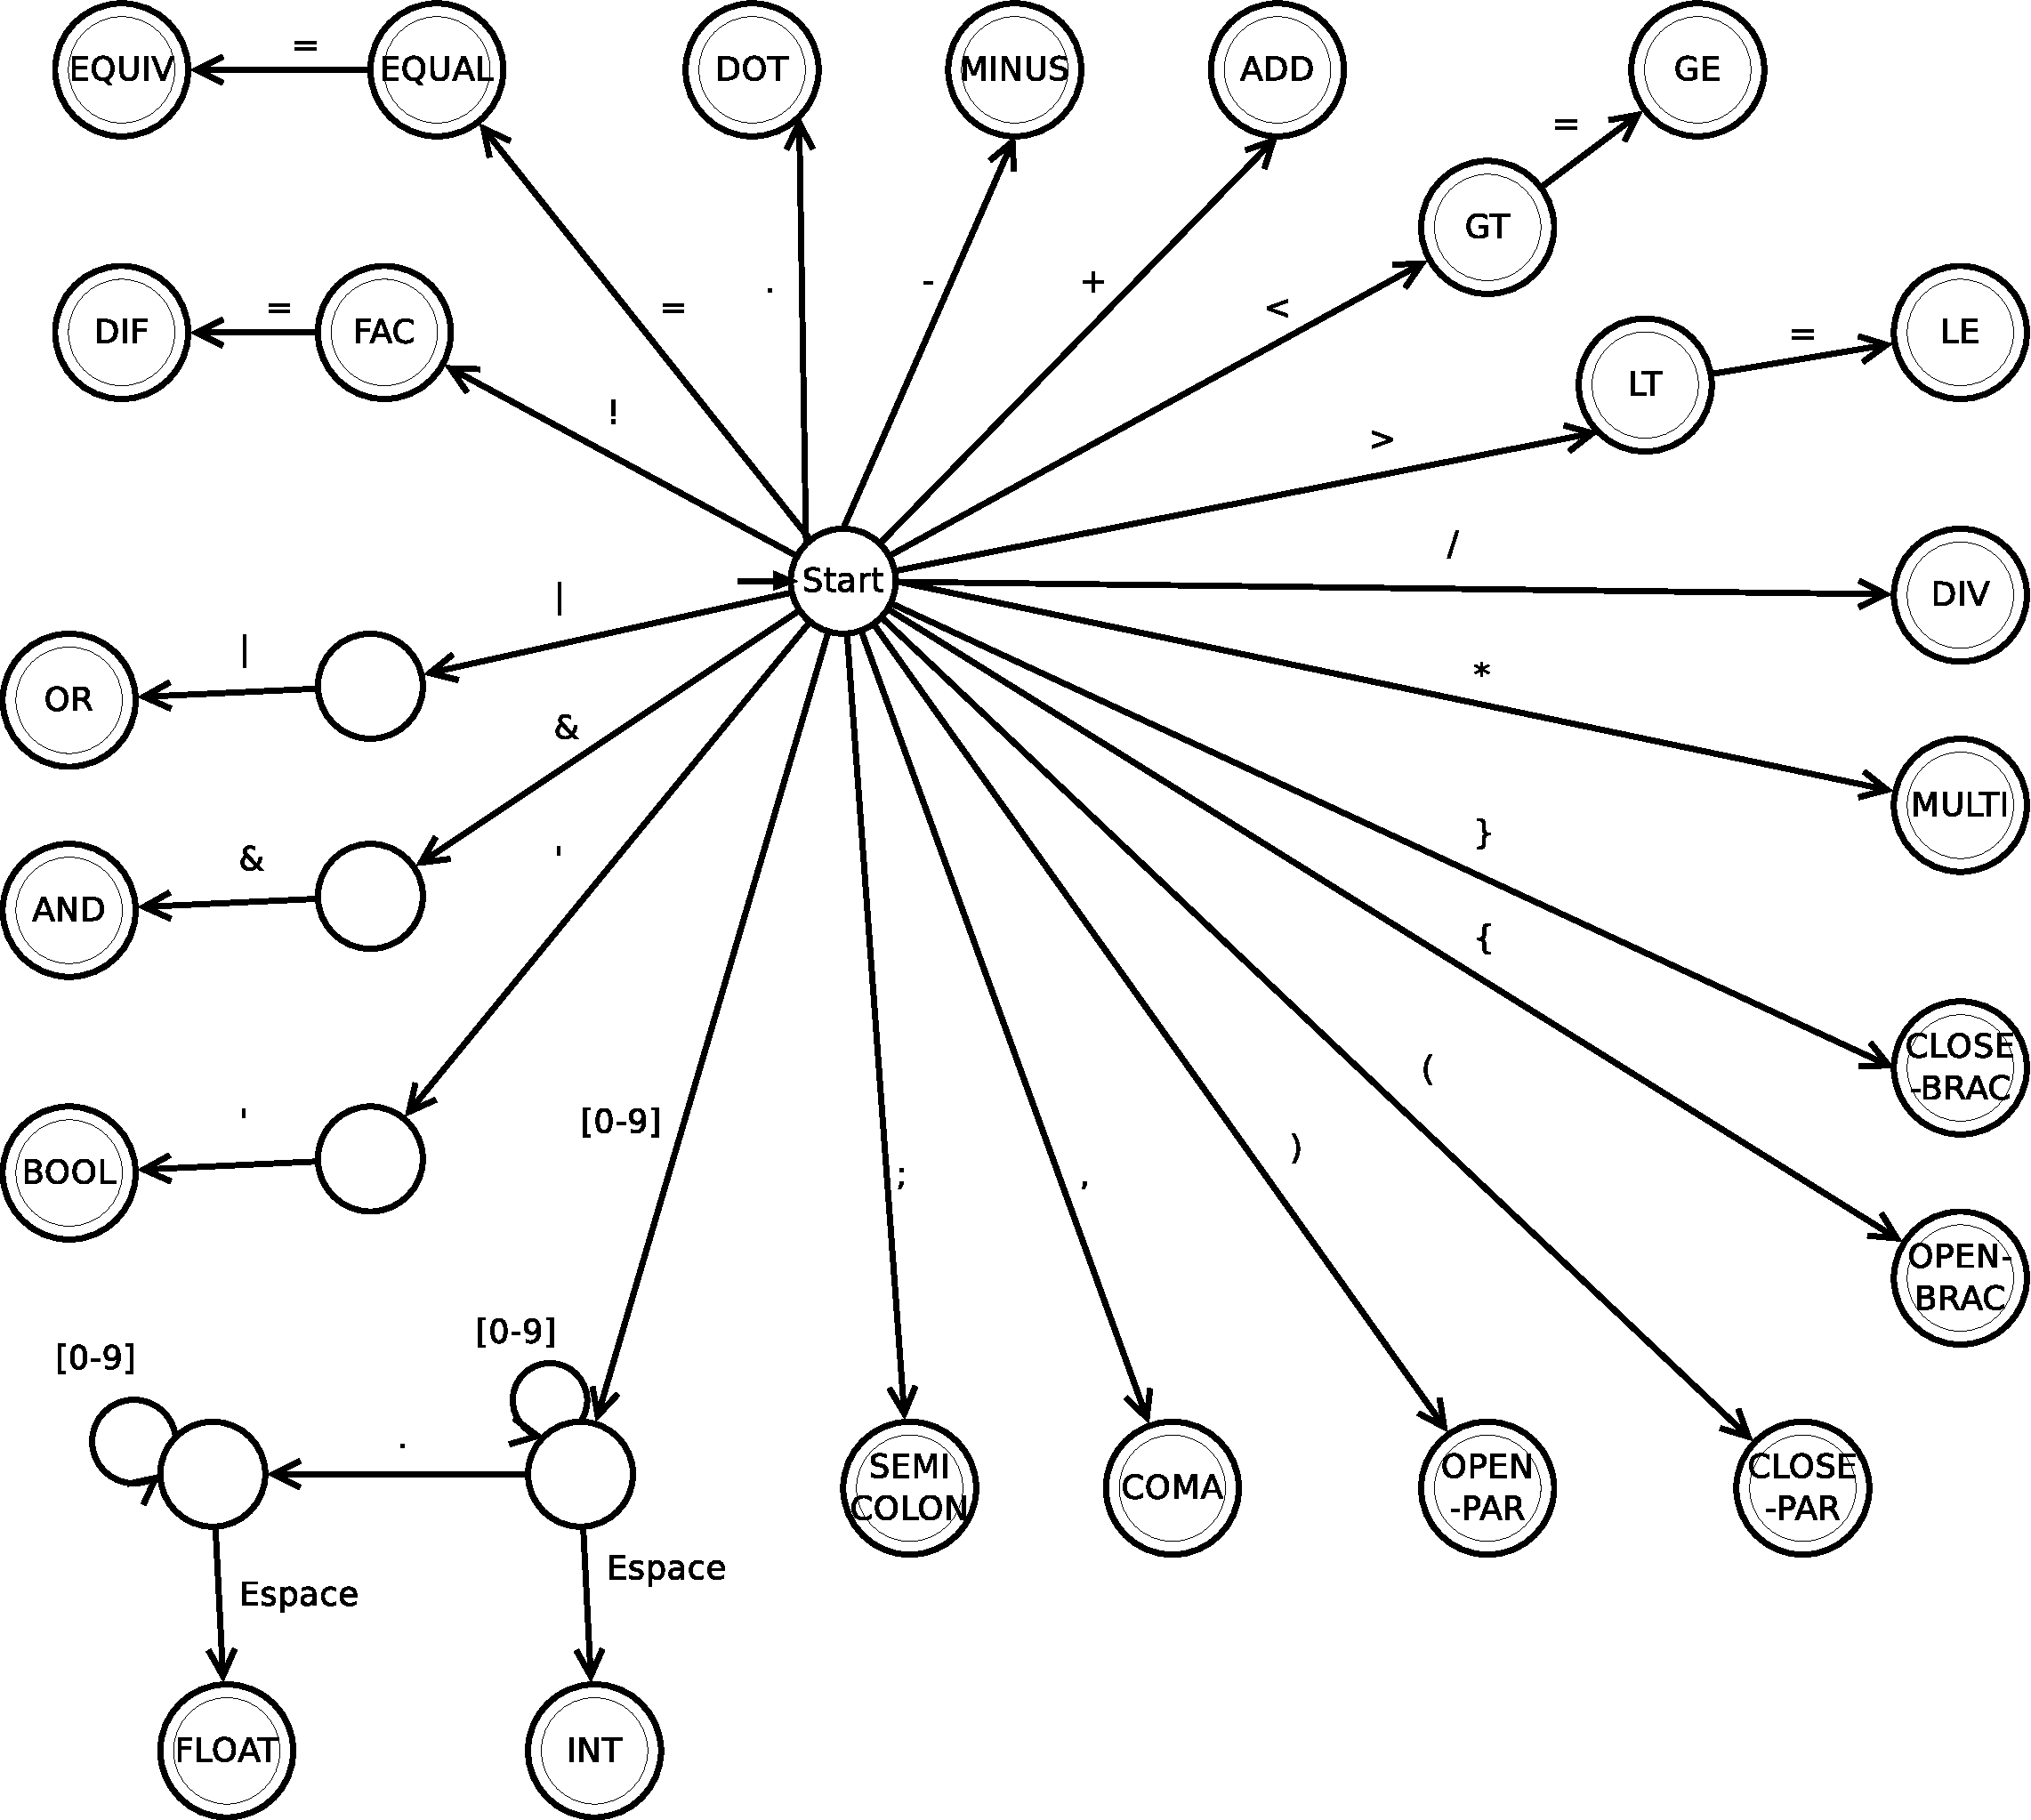
\includegraphics[width=400pt]{automate1.pdf} 
			\caption{automate "non alphabétique"}
			\label{automate1}
  \end{figure}	
  
  	Dans la figure \ref{automate2}, Les flèches bleues représentent les transitions vers l'état ID.
  
  \begin{figure}[H] \hspace*{-2cm} 
    \centering
   	  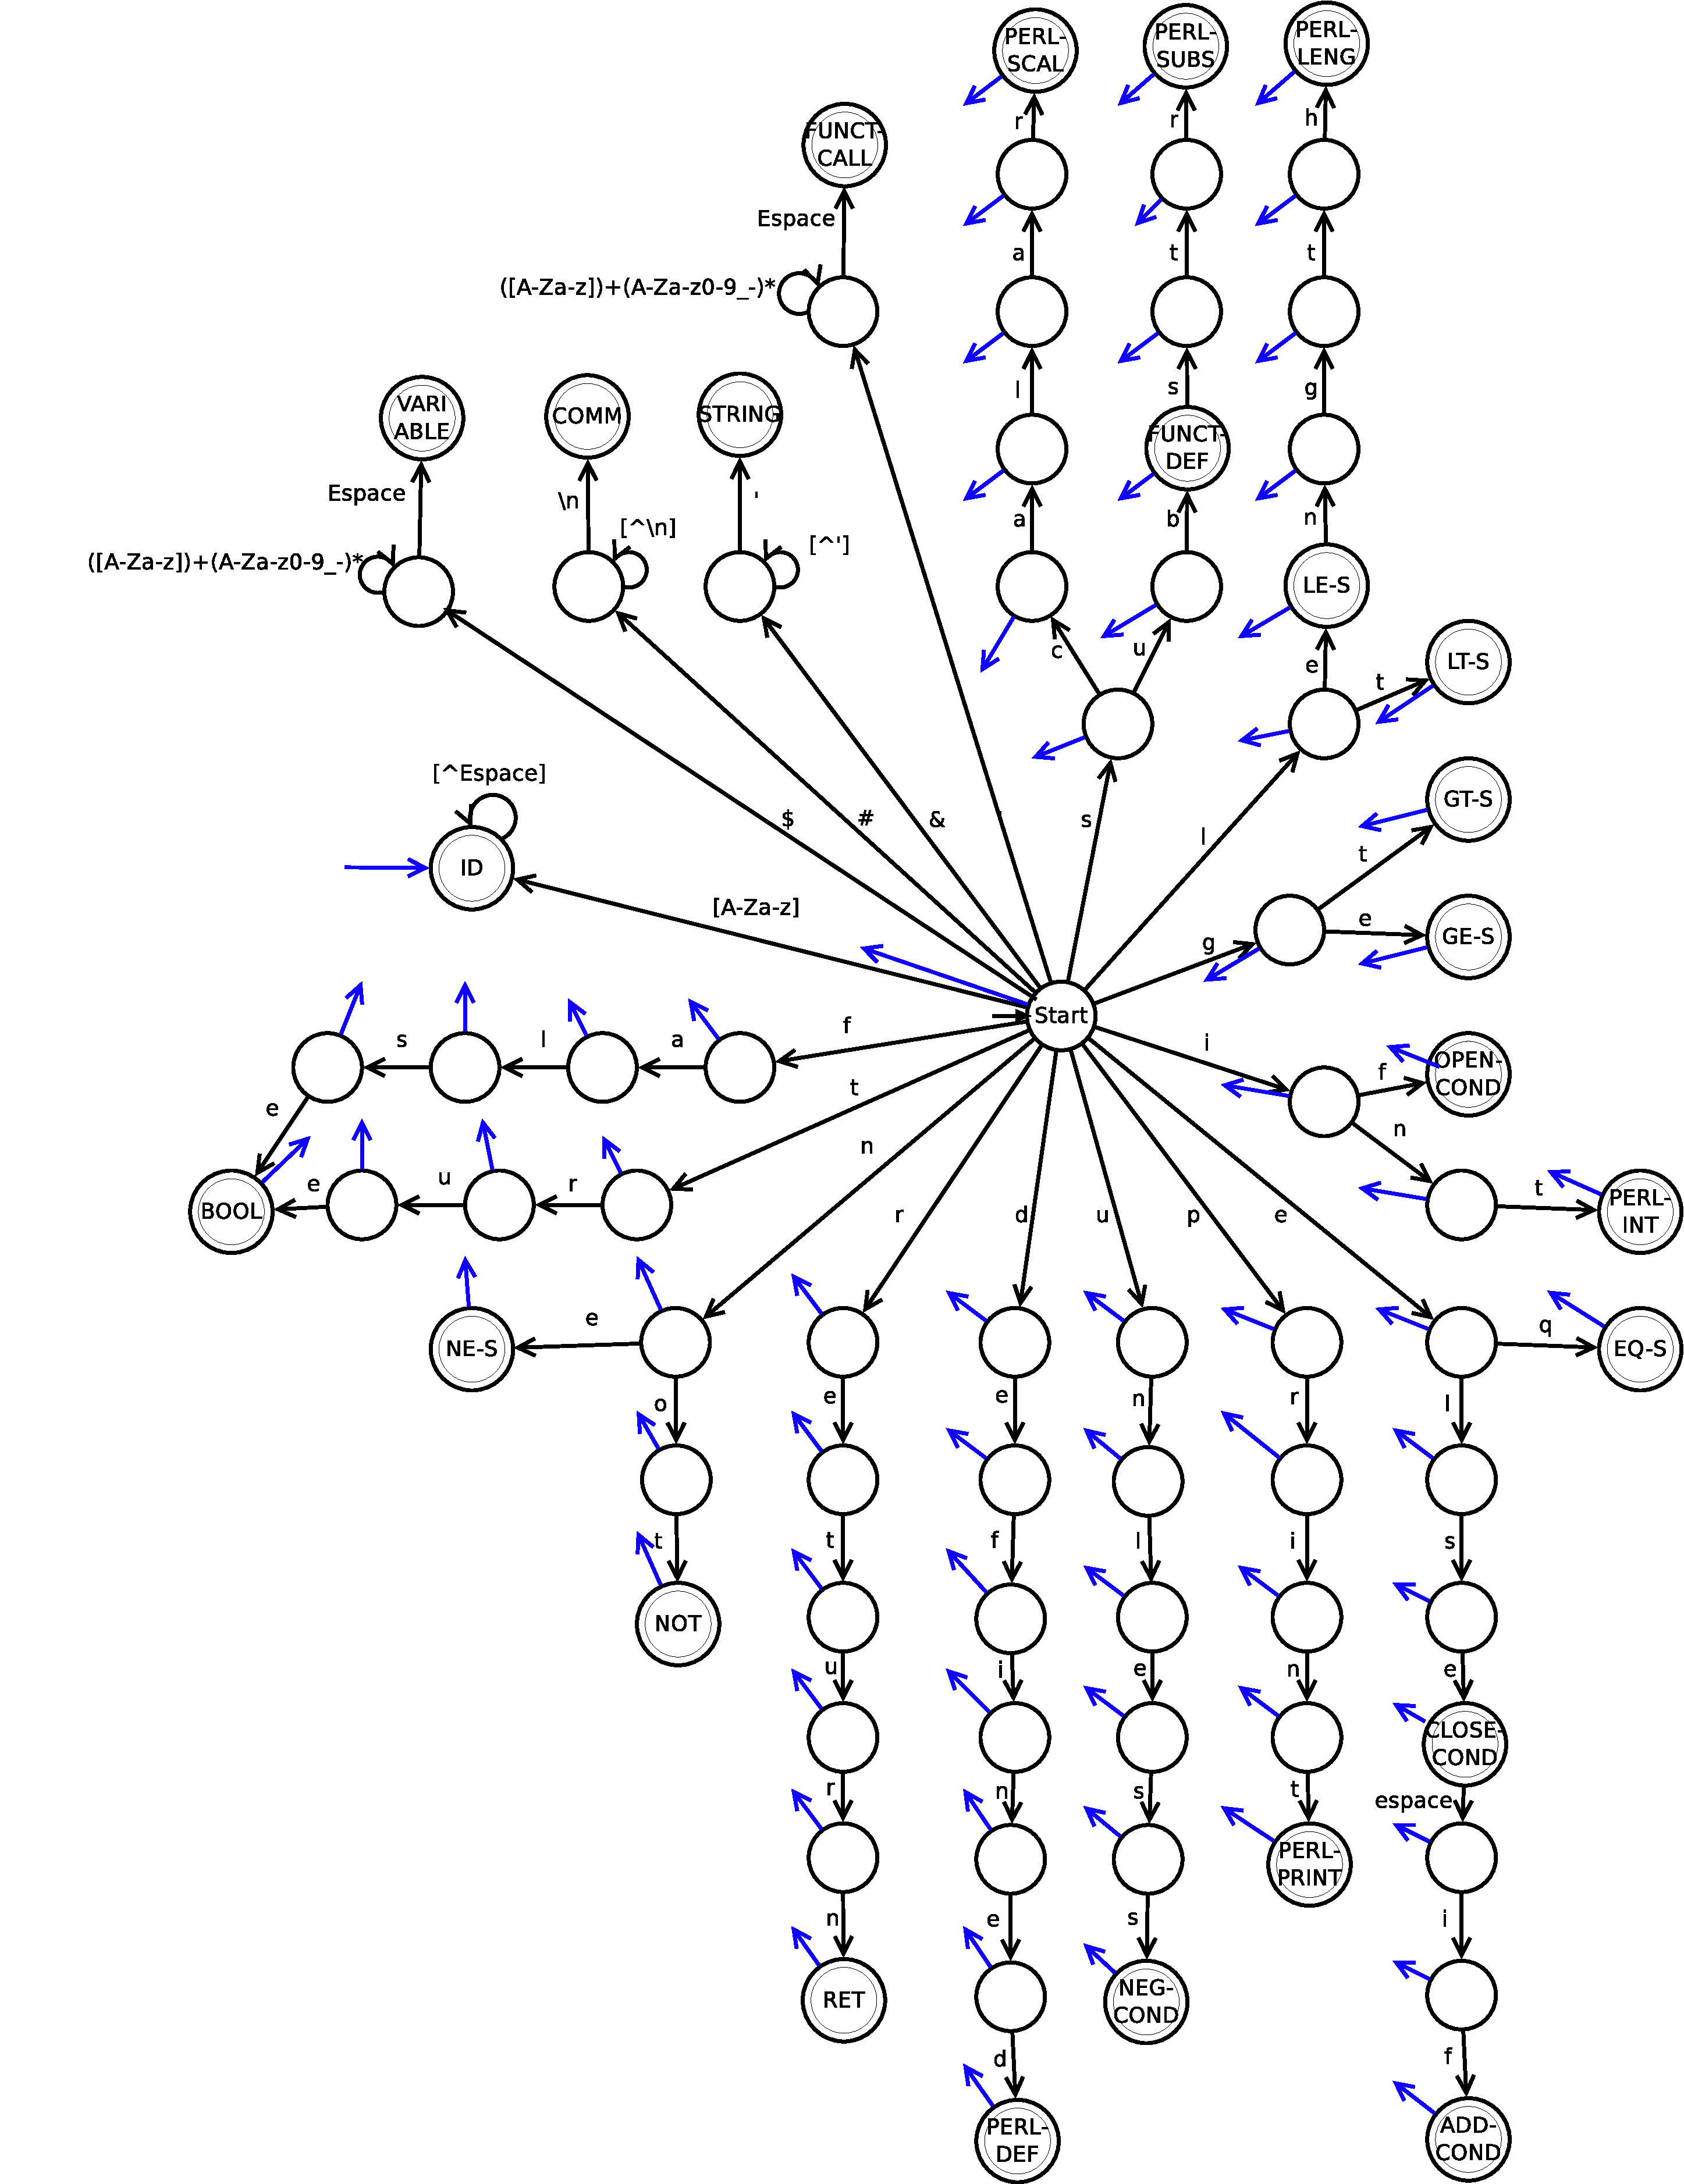
\includegraphics[width=450pt]{automate2.pdf} 
			\caption{automate "alphabétique"}
			\label{automate2}
  \end{figure}	


\pagebreak
%%%%%%%%%%%%%%%%%%%%%%%%%%%%%%%%%%%%%%%%%%%%%%%%%%%%%%%%%%%%%%%%%%%%%%%%%%%%%%%%%%%%%%%%%%%%%%%%%%%%%%%%%%%%%%%%%%%%%%%%%%%%%%%%%%%%%%%%%
%%
%%
%%	Quenstion 3 : Grammaire LL1
%%
%%
%%%%%%%%%%%%%%%%%%%%%%%%%%%%%%%%%%%%%%%%%%%%%%%%%%%%%%%%%%%%%%%%%%%%%%%%%%%%%%%%%%%%%%%%%%%%%%%%%%%%%%%%%%%%%%%%%%%%%%%%%%%%%%%%%%%%%%%%%%
\subsection{Grammaire}

	\subsubsection{Grammaire initiale}
	
	Pour rappel, voici la grammaire donnée initialement :\\
	
	
\hspace{-3.0cm}\begin{tabular}{rl}
$<$PROGRAM$>$		& $\rightarrow$ $<$FUNCT-LIST$>$ $<$INSTRUCT-LIST$>$\\
					& $\rightarrow$ $<$FUNCT-LIST$>$\\
					& $\rightarrow$ $<$INSTRUCT-LIST$>$\\
					
					
$<$FUNCT-LIST$>$	& $\rightarrow$ $<$FUNCT$>$ \\
					& $\rightarrow$ $<$FUNCT-LIST$>$ $<$FUNCT$>$\\
					
$<$FUNCT$>$			& $\rightarrow$ funct-def id open-par $<$FUNCT-ARG$>$ close-par open-brac $<$INSTRUCT-LIST$>$ close-brac \\

					
$<$FUNCT-ARG$>$		& $\rightarrow$ open-par $<$ARG-LIST$>$ close-par\\

$<$ARG-LIST$>$		& $\rightarrow$ $<$ARG-LIST$>$ coma variable \\ 
					& $\rightarrow$ variable\\ 
					& $\rightarrow$ epsilon \\

$<$INSTRUCT-LIST$>$	& $\rightarrow$ $<$INSTRUCT-LIST$>$ $<$INSTRUCT$>$ semicolon\\
					& $\rightarrow$ $<$INSTRUCT$>$ semicolon\\
					
$<$FUNCT-CALL$>$	& $\rightarrow$ funct-name $<$FUNCT-CALL-ARG$>$\\

$<$FUNCT-CALL-ARG$>$& $\rightarrow$ $<$FUNCT-CALL-ARG$>$ coma $<$EXP$>$\\
					& $\rightarrow$ $<$EXP$>$\\
					& $\rightarrow$ epsilon\\

$<$INSTRUCT$>$		& $\rightarrow$ variable equal $<$EXP$>$\\
					& $\rightarrow$ $<$EXP$>$\\
					& $\rightarrow$ ret $<$EXP$>$\\
					& $\rightarrow$ $<$COND$>$\\
					
$<$COND$>$			& $\rightarrow$ open-cond $<$EXP$>$ open-brac $<$INSTRUCT-LIST$>$ close-brac $<$COND-END$>$\\



$<$COND-END$>$		& $\rightarrow$ add-cond $<$EXP$>$ open-brac $<$INSTRUCT-LIST$>$ close-brac $<$COND-END$>$ \\
					& $\rightarrow$ close-cond open-brac $<$INSTRUCT-LIST$>$ close-brac\\
					& $\rightarrow$ epsilon \\
					
$<$SIMPLE-EXP$>$	& $\rightarrow$ int \\
					& $\rightarrow$ $<$FUNCT-CALL$>$ \\
					& $\rightarrow$ variable \\
					& $\rightarrow$ string \\				

$<$EXP$>$			& $\rightarrow$ $<$SIMPLE-EXP$>$   \\
					& $\rightarrow$ open-par $<$EXP$>$ close-par\\ 
					& $\rightarrow$ $<$EXP$>$ add $<$EXP$>$ \\
					& $\rightarrow$ $<$EXP$>$ minus $<$EXP$>$ \\
					& $\rightarrow$ $<$EXP$>$ multi $<$EXP$>$ \\
					& $\rightarrow$ $<$EXP$>$ div $<$EXP$>$ \\
					& $\rightarrow$ $<$EXP$>$ equiv $<$EXP$>$ \\
					& $\rightarrow$ $<$EXP$>$ gt $<$EXP$>$ \\
					
					
\end{tabular}

\subsubsection{Suppression des symboles inutiles}

	On peut retirer les symboles non-productifs et les symboles inaccessibles. Ici tous les symboles sont utiles dont on ne peut en retirer aucun.

\subsection{Gestion des priorités et associativité}
	On veut retirer les ambiguités liées aux priorités et à l'associativité. Cela ne concerne que la règle EXP, on la transforme donc en respectant les règles de priorités et d'associativités habituelles : \\

	\begin{center}\begin{tabular}{rl}
		$<$EXP$>$			& $\rightarrow$ $<$EXP$>$ equiv $<$EXP-2$>$ \\
							& $\rightarrow$ $<$EXP$>$ gt $<$EXP-2$>$ \\ 
							& $\rightarrow$ $<$EXP-2$>$ \\
					
		$<$EXP-2$>$			& $\rightarrow$ $<$EXP-2$>$ add $<$EXP-3$>$   \\
							& $\rightarrow$ $<$EXP-2$>$ minus $<$EXP-3$>$ \\ 
							& $\rightarrow$ $<$EXP-3$>$ \\

		$<$EXP-3$>$			& $\rightarrow$ $<$EXP-3$>$ mul $<$SIMPLE-EXP$>$  \\
							& $\rightarrow$ $<$EXP-3$>$ div $<$SIMPLE-EXP$>$\\ 
							& $\rightarrow$ $<$SIMPLE-EXP$>$ \\					
	\end{tabular}\end{center}

\subsection{left factoring}
	Cela ne concerne que EXP, EXP-2, EXP-3 et PROGRAM : \\
	\begin{center}\begin{tabular}{rl}
		$<$PROGRAM$>$		& $\rightarrow$ $<$FUNCT-LIST$>$ $<$PROG-TAIL$>$\\
							& $\rightarrow$ $<$INSTRUCT-LIST$>$\\
		$<$PROG-TAIL$>$		& $\rightarrow$ $<$INSTRUCT-LIST$>$\\
							& $\rightarrow$ epsilon\\
							&\\
							&\\
		$<$EXP$>$			& $\rightarrow$ $<$EXP-2$>$ $<$EXP-TAIL$>$ \\

		$<$EXP-TAIL$>$		& $\rightarrow$ equiv $<$EXP-2$>$ $<$EXP-TAIL$>$\\
							& $\rightarrow$ gt $<$EXP-2$>$ $<$EXP-TAIL$>$\\ 
							& $\rightarrow$ epsilon \\
					
		$<$EXP-2$>$			& $\rightarrow$ $<$EXP-3$>$ $<$EXP-2-TAIL$>$ \\

		$<$EXP-2-TAIL$>$	& $\rightarrow$ add $<$EXP-3$>$ $<$EXP-2-TAIL$>$\\
							& $\rightarrow$ minus $<$EXP-3$>$ $<$EXP-2-TAIL$>$\\ 
							& $\rightarrow$ epsilon \\
					
		$<$EXP-3$>$			& $\rightarrow$ $<$SIMPLE-EXP$>$ $<$EXP-3-TAIL$>$ \\

		$<$EXP-3-TAIL$>$	& $\rightarrow$ mul $<$SIMPLE-EXP$>$ $<$EXP-3-TAIL$>$\\
							& $\rightarrow$ div $<$SIMPLE-EXP$>$ $<$EXP-3-TAIL$>$\\ 
							& $\rightarrow$ epsilon \\				
	\end{tabular}\end{center}

\subsection{Left recursion}
	Les grammaires LL(k) ne peuvent contenir de règles du type $A \rightarrow A \beta$. Cela concerne FUNCT-LIST, ARG-LIST, INSTRUCT-LIST, FUNCT-CALL-ARG : \\

	\begin{center}\begin{tabular}{rl}				
					
		$<$FUNCT-LIST$>$		& $\rightarrow$ $<$FUNCT-LIST-BEG$>$ $<$FUNCT-LIST-END$>$\\
		$<$FUNCT-LIST-BEG$>$	& $\rightarrow$ $<$FUNCT$>$ \\
		$<$FUNCT-LIST-END$>$	& $\rightarrow$ $<$FUNCT$>$ $<$FUNCT-LIST-END$>$\\
								& $\rightarrow$ EPSILON \\
								&\\
								&\\

		$<$ARG-LIST$>$			& $\rightarrow$ $<$ARG-LIST-BEG$>$ $<$ARG-LIST-END$>$\\ 
		$<$ARG-LIST-BEG$>$		& $\rightarrow$ variable\\ 
								& $\rightarrow$ epsilon \\
		$<$ARG-LIST-END$>$		& $\rightarrow$ coma variable $<$ARG-LIST-END$>$\\ 
								& $\rightarrow$ epsilon \\
								&\\
								&\\
		$<$INSTRUCT-LIST$>$		& $\rightarrow$ $<$INSTRUCT$>$ semicolon $<$INSTRUCT-LIST$>$\\
								& $\rightarrow$ epsilon\\
								&\\
								&\\

		$<$FUNCT-CALL-ARG$>$	& $\rightarrow$ $<$FUNCT-CALL-ARG-BEG$>$ $<$FUNCT-CALL-ARG-END$>$\\ 
		$<$FUNCT-CALL-ARG-BEG$>$& $\rightarrow$ $<$EXP$>$\\ 
								& $\rightarrow$ epsilon \\
		$<$FUNCT-CALL-ARG-END$>$& $\rightarrow$ coma $<$EXP$>$ $<$FUNCT-CALL-ARG-END$>$\\ 
								& $\rightarrow$ epsilon \\
	\end{tabular}\end{center}

\subsection{Suppresion des productions unitaires}
	 règle FUNCT-ARG ($<$FUNCT-ARG$>$ $\rightarrow$ open-par $<$ARG-LIST$>$ close-par) est dans ce cas\\
	On la remplace donc directement par ARG-LIST dans funct.\\
	~\\
	FUNCT devient donc : ($<$FUNCT$>$	 $\rightarrow$ funct-def id $<$ARG-LIST$>$ open-brac $<$INSTRUCT-LIST$>$ close-brac) \\
	et arg-list devient : ($<$ARG-LIST$>$  $\rightarrow$ open-ar $<$ARG-LIST-BEG$>$ $<$ARG-LIST-END$>$ close-par)\\
	supprime donc une règle pas intermédiaire peu utile


\subsection{Grammaire finale}

\hspace{-3.0cm}\begin{tabular}{rl}	
	$<$PROGRAM$>$				& $\rightarrow$ $<$FUNCT-LIST$>$ $<$PROG-TAIL$>$ \\
								& $\rightarrow$ $<$INSTRUCT-LIST$>$ \\
	$<$PROG-TAIL$>$				& $\rightarrow$ $<$INSTRUCT-LIST$>$ \\
								& $\rightarrow$ epsilon \\
						
	$<$FUNCT-LIST$>$			& $\rightarrow$ $<$FUNCT-LIST-BEG$>$ $<$FUNCT-LIST-END$>$ \\
	$<$FUNCT-LIST-BEG$>$		& $\rightarrow$ $<$FUNCT$>$ \\
	$<$FUNCT-LIST-END$>$		& $\rightarrow$ $<$FUNCT$>$ $<$FUNCT-LIST-END$>$ \\
								& $\rightarrow$ epsilon \\
	$<$FUNCT$>$					& $\rightarrow$ funct-def id $<$ARG-LIST$>$ open-brac $<$INSTRUCT-LIST$>$ close-brac \\
	$<$ARG-LIST$>$				& $\rightarrow$ open-par $<$ARG-LIST-BEG$>$ $<$ARG-LIST-END$>$ close-par\\
	$<$ARG-LIST-BEG$>$			& $\rightarrow$ variable \\
								& $\rightarrow$ epsilon \\
	$<$ARG-LIST-END$>$			& $\rightarrow$ coma variable $<$ARG-LIST-END$>$ \\
								& $\rightarrow$ epsilon \\
	$<$INSTRUCT-LIST$>$			& $\rightarrow$ $<$INSTRUCT$>$ semicolon $<$INSTRUCT-LIST$>$ \\
								& $\rightarrow$ epsilon \\
	$<$FUNCT-CALL$>$			& $\rightarrow$ funct-name open-par $<$FUNCT-CALL-ARG$>$ close-par \\
	$<$FUNCT-CALL-ARG$>$		& $\rightarrow$ $<$FUNCT-CALL-ARG-BEG$>$ $<$FUNCT-CALL-ARG-END$>$ \\
	$<$FUNCT-CALL-ARG-BEG$>$	& $\rightarrow$ $<$EXP$>$ \\
								& $\rightarrow$ epsilon \\
	$<$FUNCT-CALL-ARG-END$>$	& $\rightarrow$ coma $<$EXP$>$ $<$FUNCT-CALL-ARG-END$>$ \\
								& $\rightarrow$ epsilon \\
	$<$INSTRUCT$>$				& $\rightarrow$ variable equal $<$EXP$>$ \\
								& $\rightarrow$ ret $<$EXP$>$ \\
								& $\rightarrow$ $<$COND$>$ \\
	$<$COND$>$					& $\rightarrow$ open-cond $<$EXP$>$ open-brac $<$INSTRUCT-LIST$>$ close-brac $<$COND-END$>$ \\
	$<$COND-END$>$				& $\rightarrow$ close-cond open-brac $<$INSTRUCT-LIST$>$ close-brac \\
								& $\rightarrow$ add-cond $<$EXP$>$ open-brac $<$INSTRUCT-LIST$>$ close-brac $<$COND-END$>$ \\
								& $\rightarrow$ epsilon \\
	$<$SIMPLE-EXP$>$			& $\rightarrow$ $<$FUNCT-CALL$>$ \\
								& $\rightarrow$ variable \\
								& $\rightarrow$ int \\
								& $\rightarrow$ string \\
								& $\rightarrow$ open-par $<$EXP$>$ close-par \\
	$<$EXP$>$					& $\rightarrow$ $<$EXP-2$>$ $<$EXP-TAIL$>$ \\
	$<$EXP-TAIL$>$				& $\rightarrow$ equiv $<$EXP-2$>$ $<$EXP-TAIL$>$ \\
								& $\rightarrow$ gt $<$EXP-2$>$ $<$EXP-TAIL$>$ \\
								& $\rightarrow$ epsilon \\
	$<$EXP-2$>$					& $\rightarrow$ $<$EXP-3$>$ $<$EXP-2-TAIL$>$ \\
	$<$EXP-2-TAIL$>$			& $\rightarrow$ add $<$EXP-3$>$ $<$EXP-2-TAIL$>$ \\
								& $\rightarrow$ minus $<$EXP-3$>$ $<$EXP-2-TAIL$>$ \\
								& $\rightarrow$ epsilon \\
	$<$EXP-3$>$					& $\rightarrow$ $<$SIMPLE-EXP$>$ $<$EXP-3-TAIL$>$ \\
	$<$EXP-3-TAIL$>$			& $\rightarrow$ mul $<$SIMPLE-EXP$>$ $<$EXP-3-TAIL$>$ \\
								& $\rightarrow$ div $<$SIMPLE-EXP$>$ $<$EXP-3-TAIL$>$ \\
								& $\rightarrow$ epsilon \\
					
					
\end{tabular}


\pagebreak
%%%%%%%%%%%%%%%%%%%%%%%%%%%%%%%%%%%%%%%%%%%%%%%%%%%%%%%%%%%%%%%%%%%%%%%%%%%%%%%%%%%%%%%%%%%%%%%%%%%%%%%%%%%%%%%%%%%%%%%%%%%%%%%%%%%%%%%%%
%%
%%
%%	scanner
%%
%%
%%%%%%%%%%%%%%%%%%%%%%%%%%%%%%%%%%%%%%%%%%%%%%%%%%%%%%%%%%%%%%%%%%%%%%%%%%%%%%%%%%%%%%%%%%%%%%%%%%%%%%%%%%%%%%%%%%%%%%%%%%%%%%%%%%%%%%%%%%

\section{Scanner}

	reconnait plus de token que ceux supporté par la grammaire.\\
	because passé de grammaire complète à grammaire simplifié

\pagebreak
%%%%%%%%%%%%%%%%%%%%%%%%%%%%%%%%%%%%%%%%%%%%%%%%%%%%%%%%%%%%%%%%%%%%%%%%%%%%%%%%%%%%%%%%%%%%%%%%%%%%%%%%%%%%%%%%%%%%%%%%%%%%%%%%%%%%%%%%%
%%
%%
%%	parser
%%
%%
%%%%%%%%%%%%%%%%%%%%%%%%%%%%%%%%%%%%%%%%%%%%%%%%%%%%%%%%%%%%%%%%%%%%%%%%%%%%%%%%%%%%%%%%%%%%%%%%%%%%%%%%%%%%%%%%%%%%%%%%%%%%%%%%%%%%%%%%%%

\section{Parser}



	\subsection{Table de parsing}
	
	
	
	\subsection{First and follow}

\end{document}          
